A continuación presentaremos las técnicas mencionadas con su respectivo análisis:

\subsection{Vecinos}
El primer método que analizaremos será el de vecinos. Este consiste en rellenar los valores de cada una de las columnas
nuevas de la imagen replicando su valor más próximo. La principal ventaja de este metodo es la simpleza de su implementación, que consta unicamente de dos bucles para iterar la matriz original.

\begin{algorithm}
\begin{algorithmic}[1]\parskip=1mm
\caption{void vecinos(Matriz *image, Matriz *imageRes , int k)}
\FOR{0 \TO imageRes$\rightarrow$rows}
    \FOR{0 \TO imageRes$\rightarrow$cols}
        \STATE{imageRes$\rightarrow$at(i, j) $=$ image$\rightarrow$at(round(i/(k+1)), round(j/(k+1)))\\}
    \ENDFOR
\ENDFOR
\end{algorithmic}
\end{algorithm}

\subsection{Interpolación bilineal}
El segundo método que analizaremos será el de interpolación bilineal. En este caso, la idea consiste en generar un polinomio entre
dos puntos consecutivos de la imagen para, por medio de este, calcular los valores necesarios para la extensión. \\
Primero realizaremos el cálculo por filas y una vez calculados estos valores, repetiremos el mismo procedimiento por columnas.
Sean entonces $Q_{11}$, $Q_{12}$, $Q_{21}$, $Q_{22}$ los cuatro puntos de la imagen original sobre los que queremos interpolar, el objetivo es conseguir un polinomio P que valga lo mismo en cada uno de estos puntos y aproxime los nuevos valores intermedios. Usaremos entonces para esto el polinomio interpolador de Lagrange.

Interpolando entonces en el eje X obtenemos la siguiente formula:

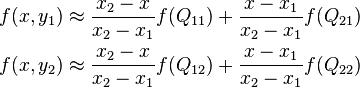
\includegraphics[scale=0.75]{imagenes/bilinealX.png}\\

Ahora, realizando el mismo procedimiento pero en el eje Y, obtenemos lo siguiente:

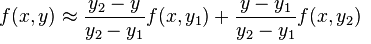
\includegraphics[scale=0.75]{imagenes/bilinealY.png}\\

Si notamos, los puntos que acompañan a las bases polinómicas de Lagrange son los mismos que calculamos sobre el eje X, por lo que podemos realizar el remplazo para llegar a una formula cerrada:

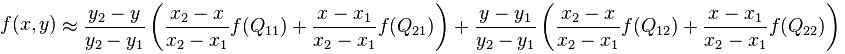
\includegraphics[scale=0.75]{imagenes/bilinealXY.png}\\

Distribuyendo los valores dentro de los paréntesis, obtenemos la ecuación final

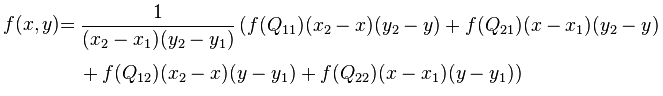
\includegraphics[scale=0.75]{imagenes/bilinealFinal.png}\\

Notese que se obtiene el mismo polinomio interpolador tanto si hace primero sobre el eje X y luego sobre el Y, como a la inversa. Ahora, gracias a este polinomio interpolador, podemos conseguir los valores de las posiciones $(x,y)$ que agregamos a nuestra imagen para realizar el zoom.

\subsection{Interpolación por Splines}
Por último nos centraremos en la interpolación por Splines. Este método, similar al anterior, requiere el cálculo de Splines (al igual que antes, por filas y luego por columnas) para obtener los valores de los casilleros a extender.
Además, en este caso, dado que la interpolación por medio de Splines trata de generar polinomios para un segmento
específico de la imagen, también analizaremos una versión en la cual el Spline calculado solo incluye los valores de un recuadro de tamaño menor, dejando de lado los valores de la imagen externos (que están influyendo sobre un polinomio que intenta interpolar valores posiblemente lejos de los suyos).

% DATOS DE SPLINES
